Pierwszą propozycją było najbardziej kompleksowe rowiązanie, czyli "Ground station". Jednym z proponowanych modeli był: DJI iPad Ground Station w/Bluetooth Module. Cechami wyróżniającymi go były:

\begin{itemize}
\item nadajnik i odbiornik 2.4 Ghz,
\item moduł Bluetooth i oprogramowanie PC Ground Station umożliwiające nawigacje,
\item dane typu stan baterii, wysokość itp.,
\item zasieg BT w pomieszczeniach do 350m,
\item moc 125mW,
\item cena 199 USD.
\end{itemize}

\begin{figure}[H]
\centering
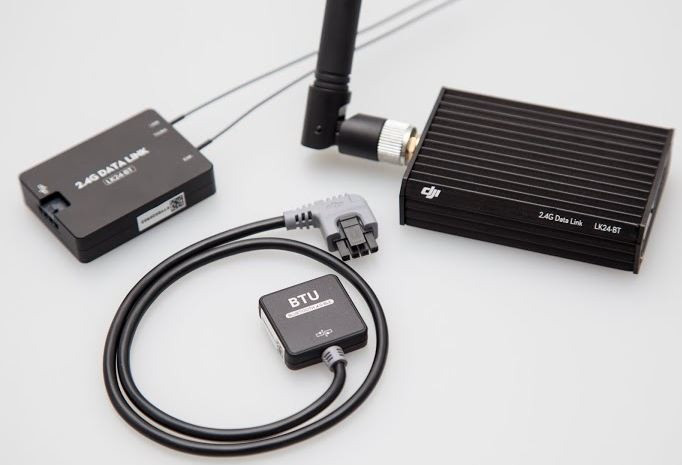
\includegraphics[width=0.7\textwidth]{./grafika/ground1.png}
\caption[DJI Ground Station]}
\end{figure}

Kolejnym zaproponowanym rozwiązaniem był: Quanum FPV Ground Station with 8” Monitor and Voltage Display, który cechował się nastepującymi elementami:

\begin{itemize}
\item rozwiązanie FPV - monitor LCD,
\item gotowe wyprowadzenia (kable, złacza) do podłaczenia anteny, sygnału video, modułu radiowego itp.,
\item nie zawiera żadnych odbiorników,
\item cena ok. 130 EUR,
\end{itemize}

\begin{figure}[H]
\centering
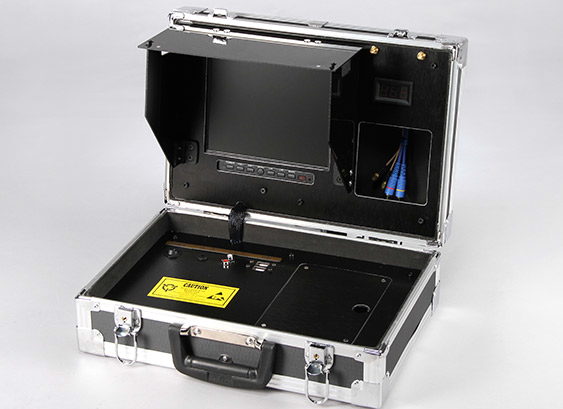
\includegraphics[width=0.7\textwidth]{./grafika/ground2.png}
\caption[Quanum FPV Ground Station]}
\end{figure}

Ostatnią alternatywą jest QGroundControl. Prezentowane rozwiązanie nie tyle jest samodzielnym produktem co niezależnym oprogramowaniem dedykowanym dla stacji PIXHAWK. Pakiet zawiera następujące elementy:

\begin{itemize}
\item Open Source - protokół MAVLink,
\item Linux Support,
\item mapy 2D/3D,
\item łatwe ustawianie punktów przelotu i manipulacja w locie,
\item przedstawianie danych telemetrycznych w czasie rzeczywistym,
\item wsparcie dla UDP i komunikacji radiowej,
\item wsparcie dla autopilota, m.in. pxIMU,
\item wsparcie dla transmisji video,
\item obsługa wielu pojazdów jednoczesnie.
\end{itemize}

\begin{figure}[H]
\centering
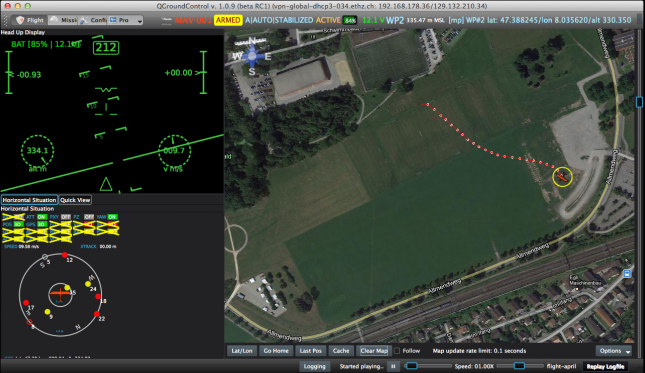
\includegraphics[width=0.7\textwidth]{./grafika/ground3.png}
\caption[QGroundControl]}
\end{figure}